Í kafla \ref{undirkafli:synidaemi-i-sql} sáum við dæmi um hvernig búa má til töflu með SQL-skipun. Hins vegar eyddum við ekki sérstaklega miklum tíma í að reyna að skilja hvernig skipunin er uppbyggð, hvað öll lykilorðin sem fram komu þýddu eða hvað er leyfilegt. Viðfangsefni kaflans sem við erum stödd í núna verður að leiðrétta þennan trassaskap og sökkva okkur í töflugerð.
\section{Að búa til töflu} % CREATE
Tökum skref aftur á bak frá og athugum hversu einfalda töflu við getum búið til. Hún er líklega eitthvað á þá leið sem sjá má á sýnidæmi \ref{sql:k3d1-create-table-fallegt}.

\begin{example}
\caption[Mjög einföld tafla]{Mjög einföld tafla. Athugum að ``NafnToflu'' og ``nafnDalks'' er ekki hluti af SQL-málinu, heldur bara dæmi um hvernig heiti á töflum og dálkum eru skilgreind.}
\label{sql:k3d1-create-table-fallegt}
\centering
\sql{sql/k3d1-create-table-fallegt.sql}
\end{example}

Skoðum þessa skipun nú mjög vandlega.
\begin{itemize}
 \item Hún hefst á að lýsa yfir hvað gera skal - hér er það \verb|CREATE TABLE|. Næst kemur nafn töflunnar fram.
 \item Þegar nafn töflunnar hefur verið gefið opnast svigi.
 \item Inni í sviganum kemur nafnið á einum dálki og orðið \verb|INTEGER|\footnote{Merkingin á þessum lykilorðum sem við höfum séð á eftir dálkheitunum, \emph{INTEGER} og \emph{VARCHAR}, útskýrist í næsta undirkafla (\ref{undirkafli:gagnagerdir}).}. Hér er einungis einn dálkur.
 \item Skipuninni lýkur á því að sviganum er lokað og semíkomma (;) sett á eftir.
\end{itemize}

Skoðum næst sýnidæmi \ref{sql:k3d2-create-table-meira-fallegt}, sem er \emph{örlítið} stærra.
\begin{example}
\caption{Einföld tafla}
\label{sql:k3d2-create-table-meira-fallegt}
\centering
\sql{sql/k3d2-create-table-meira-fallegt.sql}
\end{example}

Hér sjáum við ágætlega hvernig bæta má við öðrum dálki. Fyrsta dálklýsingin er skrifuð, síðan kemur komma, síðan fylgir næsta dálklýsing.

Athugum að engin komma er á eftir síðustu dálklýsingunni. Það er vegna þess að dálkarnir eru einungis \emph{aðskildir} með kommum, komman er ekki hluti af dálklýsingunni sjálfri.
\section{Innsetning gagna} % INSERT
\label{undirkafli:innsetning}
Þegar töflur eru búnar til með \verb|CREATE TABLE| skipun eru þær tómar. Til að fylla töflu með gögnum þarf að nota aðra skipun - \verb|INSERT|. Til að setja töluna $1$ inn í töfluna sem við bjuggum til með sýnidæmi \ref{sql:k3d1-create-table-fallegt} mætti nota \verb|INSERT| skipunina í sýnidæmi \ref{sql:k3d8-insert-einfalt}.

\begin{example}
\caption[INSERT í einfalda töflu]{INSERT í einfalda töflu. Þessi skipun setur töluna $1$ inn dálkinn \emph{nafnDalks}. Niðurstaðan er tafla \ref{tafla:insert-einfalt}.}
\label{sql:k3d8-insert-einfalt}
\centering
\sql{sql/k3d8-insert-einfalt.sql}
\end{example}

Skoðum þessa skipun í smáatriðum líka. 

\begin{itemize}
 \item Aftur hefst skipunin á því að lýsa því yfir hvað gera skal. Hér ætlum við að setja inn gögn - \verb|INSERT|. Við ætlum að setja gögnin inn í eitthvað, svo við segjum \verb|INSERT INTO|.
 \item Næst kemur nafn töflunnar sem gögnin eiga að fara í. %Gagnagrunnskerfið getur ekki giskað á hvert gögnin eiga að fara. %Við verðum að taka það fram.
 \item Svigi opnast, nafn dálksins sem gögnin eiga að fara inn í er skrifað og sviginn lokast.\footnote{Strangt til tekið er hægt að sleppa þessum sviga. Gagnagrunnskerfið reynir þá að setja gögnin inn í þá dálka sem það finnur í töflunni. Þessar ágiskanir geta verið til vandræða, betra er að venja sig á að taka dálkheitin alltaf fram.}
 \item Að lokum segjum við hvað við ætlum að setja inn. Það eru gögn (eða ``gildi'', \verb|VALUES|). Gögnin sem við ætlum að setja inn er ein lína, sem við afmörkum með svigum. Línan samanstendur af einni tölu. Sem fyrr lokum við skipuninni með semíkommu.
\end{itemize}

\begin{table}
\centering
\caption[Eftir einfalt INSERT]{Niðurstaðan eftir að sýnidæmi \ref{sql:k3d1-create-table-fallegt} og \ref{sql:k3d8-insert-einfalt} hafa verið keyrð - ofurlítil tafla með einum dálki og einni línu af gögnum.}
\label{tafla:insert-einfalt}
\begin{tabular}{l}
\toprule
nafnDalks\\
\midrule
1\\
\bottomrule
\end{tabular}
\end{table}

Mikilvægt er að vita að \verb|INSERT| skipun setur alltaf inn \emph{heila línu} af gögnum í töfluna. Sé taflan með fleiri en einn dálk (Flestar töflur sem ekki eru gagnslausar hafa fleiri en einn dálk.) þarf að skilgreina öll gögnin í einu. Sýnidæmi \ref{sql:k3d9-insert-margir-dalkar} er dæmi um slíkt.

\begin{example}
\caption[INSERT í tvo dálka í einu]{INSERT í tvo dálka í einu. Þessi skipun setur tölurnar $1$ og $2$ inn í sömu línu. Niðurstaðan er tafla \ref{tafla:insert-margir-dalkar}.}
\label{sql:k3d9-insert-margir-dalkar}
\centering
\sql{sql/k3d9-insert-margir-dalkar.sql}
\end{example}

\begin{table}
\centering
\caption[Eftir INSERT á línu]{Niðurstaðan eftir að sýnidæmi \ref{sql:k3d2-create-table-meira-fallegt} og \ref{sql:k3d9-insert-margir-dalkar} hafa verið keyrð. Tafla með tveimur dálkum og einni línu af gögnum.}
\label{tafla:insert-margir-dalkar}
\begin{tabular}{ll}
\toprule
nafnFyrstaDalks&nafnAnnarsDalks\\
\midrule
1&2\\
\bottomrule
\end{tabular}
\end{table}
Til að skrifa meira en eina línu af gögnum inn í gagnagrunn má keyra \verb|INSERT| skipun oftar en einu sinni. Væri skipunin í sýnidæmi \ref{tafla:insert-margir-dalkar} keyrð tvisvar myndi línan sem hún lýsir vera tvítekin í töflunni.

Það að skrifa alla \verb|INSERT INTO| romsuna upp upp á nýtt fyrir hverja línu sem setja skal inn getur verið þreytandi. Þess vegna býður MySQL upp á leið til að setja inn margar línur í einu. Við sjáum dæmi um það í sýnidæmi \ref{sql:k3d10-insert-margar-linur}.

\begin{example}
\caption[INSERT í tvo dálka í einu]{INSERT í tvo dálka í einu. Þessi skipun setur tölurnar $1$ og $2$ inn í eina línu og tölurnar $3$ og $4$ í þá næstu. Niðurstaðan er tafla \ref{tafla:insert-margar-linur}.}
\label{sql:k3d10-insert-margar-linur}
\centering
\sql{sql/k3d10-insert-margar-linur.sql}
\end{example}

\begin{table}
\centering
\caption[Eftir INSERT á tveimur línum]{Niðurstaðan eftir að sýnidæmi \ref{sql:k3d2-create-table-meira-fallegt} og \ref{sql:k3d10-insert-margar-linur} hafa verið keyrð. Tafla með tveimur dálkum og tveimur línum af gögnum.}
\label{tafla:insert-margar-linur}
\begin{tabular}{ll}
\toprule
nafnFyrstaDalks&nafnAnnarsDalks\\
\midrule
1&2\\
3&4\\
\bottomrule
\end{tabular}
\end{table}

\section{Algengar gagnagerðir: Tölur og texti} % INTEGER (INT), VARCHAR, CHAR
\label{undirkafli:gagnagerdir}
Einni stórri spurningu um \verb|CREATE TABLE| dæmin framar í þessum kafla er enn ósvarað - hvað er þetta \verb|INTEGER|?

Integer er dæmi um svokallaða gagnagerð\footnote{e. \emph{data type}}. Nánar til tekið er þetta gagnagerð sem táknar heiltölur, tölur eins og töluna $1$, töluna $-256$ og allar tölur sem við höfum sett inn í töflur framar í bókinni. Þegar \verb|INTEGER| kemur fyrir í dálkskilgreiningu erum við sem sagt að segja gagnagrunnskerfinu að við munum einungis geyma heiltölur í þessum dálki.

Skoðum nokkrar helstu gagnagerðir í MySQL og hvenær við notum þær.
\subsection{Heiltölur - INTEGER}
Fram hefur komið að \verb|INTEGER| dálkur geymi heiltölur. Hann tekur ekki við kommutölum.\footnote{Í stað \emph{INTEGER} má skrifa styttinguna \emph{INT}, sem hefur sömu áhrif.}

Lægsta talan sem slíkur dálkur getur geymt er $-2147483648$ og sú hæsta $2147483647$. Ástæðan fyrir því að lægri og hærri tölur en þessar valda villum er sú að MySQL notar einungis fjögur bæti til að geyma hverja heiltölu - hærri og lægri tölur komast ekki fyrir í svo litlu geymsluplássi.

Sé nauðsynlegt að geyma tölur sem ekki passa inn á þetta bil má nota gagnagerðina \verb|BIGINT| í stað \verb|INTEGER|. Slíkur dálkur geymir einnig heiltölur, en hefur átta bæti til að geyma hverja tölu. \verb|BIGINT| dálkur getur því geymt mun stærri (eða ``lengri'') tölur.

Sé vitað að tölurnar sem fara inn í dálkinn séu allar mjög litlar um sig má nota gagnagerðirnar \verb|TINYINT|, \verb|SMALLINT| og \verb|MEDIUMINT| í MySQL. Þær taka hver um sig $1$, $2$ og $3$ bæti til að geyma hverja tölu. Sjaldnast er ástæða til að nota þessar gagnagerðir í dag. Tafla þyrfti að innihalda tugi milljóna raða\footnote{Reyndar eru í dag til gagnagrunnstöflur sem innihalda \emph{hundruðir milljarða} raða.} til að plásssparnaðurinn gæti skipt máli á nútíma tölvukerfum.

\begin{table}
\centering
\caption[Heiltöludálkar]{Heiltölugagnagerðir í MySQL og stærðir þeirra.}
\label{tafla:heiltolur}
\begin{tabular}{llll}
\toprule
Nafn&Stærð í&Lægsta gildi&Hæsta gildi\\
&bætum&&\\
\midrule
\verb|TINYINT|&1&$-128$&$127$\\
\verb|SMALLINT|&2&$-32768$&$32767$\\
\verb|MEDIUMINT|&3&$-8388608$&$8388607$\\
\verb|INT|&4&$-2147483648$&$2147483647$\\
\verb|BIGINT|&8&$-9223372036854775808$&$9223372036854775807$\\
\bottomrule
\end{tabular}
\end{table}

Ef sérstök skilyrði koma ekki upp er best og einfaldast að halda sig við \verb|INTEGER| til að geyma heiltölur. Þetta getur sérstaklega borgað sig ef seinna reynist nauðsynlegt að færa gagnagrunninn á milli gagnagrunnskerfa - sum gagnagrunnskerfi styðja ekki allar gagnagerðirnar sem MySQL býður upp á. Gamla góða \verb|INTEGER| er hins vegar alltaf til staðar.

\newthought{Íslenskar kennitölur} eru varhugaverðar. Freistandi getur verið að geyma kennitölur í heiltöludálkum. Þær eru jú kommulausar tölur, ekki satt? Nokkur atriði leiða þó til þess að þær passa ekki mjög vel í slíka dálka.

\begin{itemize}
 \item Stærsta tala sem hægt er að geyma í venjulegum \verb|INTEGER| dálki er $2147483647$. Það þýðir að kennitölur allra sem fæddir eru á 22. degi mánaðar eða seinna komast ekki fyrir í dálkinum! \verb|BIGINT| þyrfti að nota.
 \item Kennitölur eru ekki notaðar eins og flestar tölur. Þær eru t.d. ekki lagðar saman eða bornar saman með $<$ og $>$ virkjum. Við þurfum oftar að skoða ákveðna stafi í kennitölunni (t.d. fimmta og sjötta stafinn til að komast að fæðingarári) frekar en stærð tölunnar sjálfrar.
 \item Kennitölur eru venjulega skrifaðar með bandstrikum, sem eiga ekki heima í heiltöludálki.
\end{itemize}
Vænlegra er að nota \verb|CHAR| dálk til að geyma kennitölur. Lítum á þá gagnagerð í næsta kafla!

\subsection{Texti - VARCHAR og CHAR}
Í forritun lítum við oftast á texta sem safn af stöfum, SQL er hér engin undantekning. Slíkt safn er kallað strengur\footnote{e. \emph{string}}. \verb|'Ari'|, \verb|'Ari sá sól'| og \verb|'Ari á 10 krónur'| eru allt dæmi um strengi. 

Eins og sjá má eru strengir afmarkaðir með gæsalöppum. Mikilvægt er að gleyma þeim ekki þegar strengir eru slegnir inn (sjá kafla \ref{undirkafli:innsetning}). Þær eru aðalleiðin sem gagnagrunnskerfið hefur til að vita hvort að um streng eða dálkheiti sé að ræða. 

Venja er að nota einfaldar gæsalappir (\verb|'|) í SQL til að afmarka strengi. Tvöfaldar gæsalappir (\verb|"|) virka líka í MySQL.

Talað er um að strengur hafi ákveðna \emph{lengd}. Lengd strengs er fjöldi stafa í strengnum, að bilum meðtöldum. Gæsalappirnar eru ekki taldar með, þær umlykja strenginn en eru ekki hluti af honum. Þannig er \verb|'Ari'| strengur af lengd 3, \verb|'Ari sá sól'| er strengur af lengd 10.

Strengir geta innihaldið næstum hvaða stafi sem er, líka tölustafi. \verb|'Ari á 10 krónur'| er löglegur strengur. Strengur getur meira að segja innihaldið ekkert nema tölustafi. \verb|"10"| er strengur, $10$ er heiltala.

\newthought{Til að geyma texta} höfum við nokkrar gagnagerðir, líkt og við höfum nokkrar gagnagerðir til að geyma heiltölur. Þær helstu eru \verb|CHAR| og \verb|VARCHAR|. ``Char'' stendur hér fyrir enska orðið ``character'', sem þýða má sem ``stafur''. ``Var'' í \verb|VARCHAR| stendur fyrir ``variable''. 

Þegar \verb|CHAR| og \verb|VARCHAR| gagnagerðirnar eru notaðar þurfum við að taka fram hversu langa strengi dálkurinn á að geta tekið við\footnote{Oft er talað um ``breidd'' á þessum dálkum. Til að strengur af lengd $5$ komist inn í dálk þarf dálkurinn að vera $5$ stafa breiður.}. Þetta er gert með því að setja hámarkslengdina inn í sviga. \verb|CHAR(3)| er dálkur sem tekur við strengjum af lengd 3.

Sé strengur sem er of langur settur inn í \verb|CHAR| eða \verb|VARCHAR| dálk er klippt af hægri enda hans svo að hann passi. Væri t.d. reynt að geyma \verb|'Ari sá sól'| í \verb|CHAR(5)| dálk væri útkoman \verb|'Ari s'|. 

Munurinn á \verb|CHAR| og \verb|VARCHAR| kemur fyrst og fremst fram þegar of \emph{stuttir} strengir eru settir inn í dálkinn. 
\begin{itemize}
 \item Sé strengur styttri en breidd \verb|CHAR| dálks sem hann er settur inn í er bilum bætt við hægri enda strengsins svo hann passi nákvæmlega. Þannig yrði strengurinn \verb|'Ari sá sól'| að \verb|'Ari sá sól     '| væri hann settur inn í \verb|CHAR(15)| dálk.
 \item Sé strengur sem er of stuttur settur inn í \verb|VARCHAR| dálk er hann einfaldlega geymdur eins og hann er. \verb|VARCHAR| dálkur getur geymt ``of stutta'' strengi.
\end{itemize}
\verb|CHAR| dálkur getur verið að hámarki 255 stafir að breidd. \verb|VARCHAR| dálkur getur verið allt að 65.535 stafa breiður.

Hljómi \verb|VARCHAR| hér eins og almennt gagnlegri gagnagerð er það líklega vegna þess að það er rétt. \verb|VARCHAR| eyðir minna plássi og breytir strengjum ekki að óþörfu. \verb|CHAR| dálkar eru gagnlegir þegar vitað er fyrirfram að allir strengir sem eiga að fara inn í dálkinn séu af sömu lengd eða ef seinni tíma vinnsla krefst þess að gögnin séu sjálum sér mjög samkvæm. Leiki vafi á er einfaldast að nota bara \verb|VARCHAR|.
\begin{marginfigure}
\caption[CHAR og VARCHAR]{Hvernig CHAR og VARCHAR dálkar geyma texta. Talan til vinstri táknar lengd strengsins eins og hann er geymdur.}
\label{mynd:char-varchar}
\centering
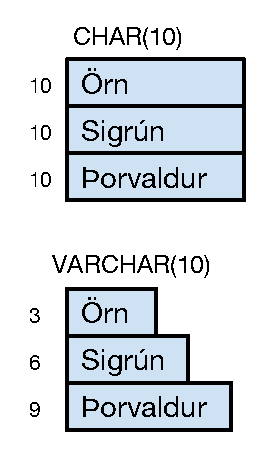
\includegraphics[width=\linewidth]{myndir/char-varchar}
\end{marginfigure}

\newthought{Mjög langur texti} getur verið erfiður í meðförum. Sé ætlunin t.d. að geyma bækur, bloggfærslur eða fréttagreinar í gagnagrunni, hversu stóran \verb|VARCHAR| dálk þyrfti til að halda utan um textann? Svarið er: Of stóran.

MySQL býður upp á aðrar gagnagerðir sem eru meira viðeigandi fyrir slíka vinnslu - hér eru helstar \verb|TEXT| og \verb|LONGTEXT|. \verb|LONGTEXT| dálkur er fær um að geyma strengi sem eru allt að 4 GiB að lengd.

Sé ætlunin að geyma upplýsingar sem almennt eru af skynsamlegri stærð, t.d. mannanöfn, þá er hagkvæmara að nota \verb|VARCHAR| dálk.

\section{Dæmi um töflur með tölum og texta}
Ýmsar töflur má búa til með tölum og texta. Fyrsta taflan sem við sáum, tafla \ref{tafla:starfsmenn-ts}, er dæmi um slíka töflu. Lítum á nokkur fleiri dæmi.

\begin{figure}
\caption[High Score tafla]{``High score'' tafla fyrir tölvuleik. Fyrir nokkrum áratugum litu high score listar í spilakössum yfirleitt út á þennan hátt. Hver lína samanstóð af þremur upphafsstöfum og stigafjölda. Hana mætti búa til með skipuninni í sýnidæmi \ref{sql:k3d4-high-score}.}
\label{mynd:high-score}
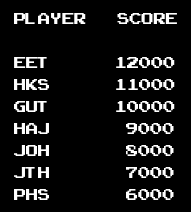
\includegraphics{myndir/high-score}
\end{figure}

\begin{example}
\caption[High Score tafla]{High score taflan á mynd \ref{mynd:high-score} búin til með SQL-skipun. Hér vitum við að spilararnir nota alltaf nákvæmlega þrjá upphafsstafi til að auðkenna sig, svo \emph{CHAR} dálkur er viðeigandi. Stigin sjálf eru geymd í \emph{INTEGER} dálki.}
\label{sql:k3d4-high-score}
\centering
\sql{sql/k3d4-high-score.sql}
\end{example}

\begin{figure}
\caption[Matseðill]{Hamborgaramatseðill á veitingastað. Töflur geta litið út á ýmsan hátt. Matseðil af þessari gerð mætti geyma í gagnagrunni, þó að hann líti e.t.v. ekki út eins og tafla við fyrstu sýn. Töflu sem heldur utan um upplýsingarnar á honum má sjá á sýnidæmi \ref{sql:k3d5-matsedill}. }
\label{mynd:matsedill}
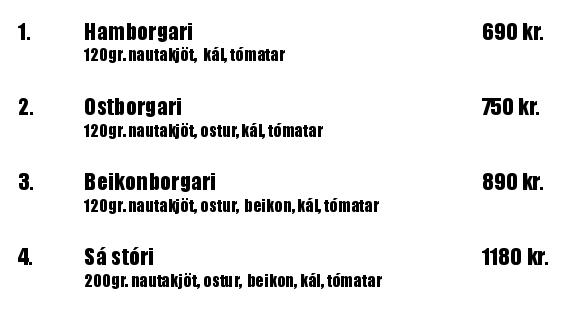
\includegraphics[width=\textwidth]{myndir/matsedill}
\end{figure}

\begin{example}
\caption[Matseðill]{SQL-framsetning á matseðlinum á mynd \ref{mynd:matsedill}. Við gerum ráð fyrir að lýsingin á réttinum þurfi meira pláss en nafn hans.}
\label{sql:k3d5-matsedill}
\centering
\sql{sql/k3d5-matsedill.sql}
\end{example}

\section{Fleiri gagnagerðir}
Þó að ýmislegt sé hægt að gera með einungis texta og heiltölum, þá býður MySQL upp á mun fleiri gagnagerðir. Lítum stuttlega á nokkrar.
\subsection{Tugabrot - DECIMAL}
Til að geyma tugabrot (kommutölur, t.d. $1,5$ og $5,2$) dugar \verb|INTEGER| dálkur ekki. Til þess getum við notað \verb|DECIMAL| dálk.

Til að búa til \verb|DECIMAL| dálk þurfum við að skilgreina tvær tölur. Sú fyrri er heildarfjöldi tölustafa sem mega vera í tölunni, sú seinni er fjöldi tölustafa ``hægra megin'' við kommuna. Þannig myndi \verb|DECIMAL(5,2)| dálkur passa akkúrat utan um töluna $123,45$.

\begin{table}
\centering
\caption[Eldsneyti]{Eldsneytisverð á bensínstöð. \emph{DECIMAL} dálkur er notaður til að halda utan um bensínverðið með nákvæmlega 1 aukastaf.}
\label{tafla:eldsneyti}
\begin{tabular}{lr}
\toprule
Gerð&Verð (kr.)\\
\midrule
95 oktan&$252,9$\\
Dísel&$242,3$\\
Vélaolía&$174,3$\\
98 oktan&$298,9$\\
\bottomrule
\end{tabular}
\end{table}

\begin{example}
\caption[Eldsneytisverð]{SQL-framsetning á eldsneytisverðinu í töflu \ref{tafla:eldsneyti}. Verðið er geymt í dálki sem tekur við tugabroti með fjóra markverða stafi, þar af einum fyrir aftan kommu. Athugum að \emph{INSERT} skipunin tekur við tölum á ensku formi, sem notar punkta þar sem kommur eru notaðar í íslensku (og öfugt). Væri reynt að setja tugabrotið inn með kommu væri það túlkað sem skipting á milli dálka!}
\label{sql:k3d6-eldsneyti}
\centering
\sql{sql/k3d6-eldsneyti.sql}
\end{example}

\subsection{Rauntölur - DOUBLE}
Það að þurfa að taka fram stærð talna getur verið mjög takmarkandi. Hvað ef skali talnanna er mjög mismunandi eða ef geyma þarf gríðarlega ``langar'' tölur? 

Massi sólarinnar er í kringum $1988550000000000000000000000000$ kg. Þessi tala passar ekki í nokkurn \verb|INTEGER| dálk - við þurfum að leita að öðrum lausnum.

\verb|DOUBLE| gagnagerðin getur geymt flestar tölur. Gallinn er sá að tölurnar í \verb|DOUBLE| dálki eru geymdar sem svokallaðar fleytitölur\footnote{e. \emph{floating point numbers}}, sem eru ekki fullkomlega nákvæmar. Þessi ónákvæmni er oftast afar smá, en getur verið til vandræða. Betra er að nota nákvæmar gagnagerðir (t.d. \verb|INTEGER| eða \verb|DECIMAL|) sé það mögulegt.

\begin{table}
\centering
\caption[Plánetur utan sólkerfisins.]{Nokkrar plánetur utan sólkerfisins sem líkjast jörðinni að einhverju leyti.}
\label{tafla:planetur}
\begin{tabular}{lll}
\toprule
Nafn&Fjarlægð (m)&Massi (kg)\\
\midrule
Gliese 667 Cc&$2,1475\cdot 10^{17}$&$2,6218\cdot10^{25}$\\
Kepler-62e   &$1,1353\cdot 10^{19}$&$2,1321\cdot10^{25}$\\
Tau Ceti e   &$1,1263\cdot 10^{17}$&$2,5680\cdot10^{25}$\\
Gliese 581 d &$1,9110\cdot 10^{17}$&$4,1686\cdot10^{25}$\\
\bottomrule
\end{tabular}
\end{table}

\begin{example}
\caption[Plánetur]{SQL-tafla sem haldið getur utan um pláneturnar í töflu \ref{tafla:planetur}. Fjarlægð þeirra frá okkar sólkerfi (í metrum) og massi þeirra (í kílóum) eru mjög óþjálar tölur, sem krefjast fleytitalna.}
\label{sql:k3d7-planetur}
\centering
\sql{sql/k3d7-planetur.sql}
\end{example}

\subsection{Dagsetningar - DATE}

\subsection{Rökbreytur - BOOLEAN}

\section{Tóm gildi} % NULL, NOT NULL
Hvað gerum við ef við þekkjum ekki 

Sérstakt lykilorð er notað í SQL til að tákna það að ákveðið gildi sé óþekkt eða ekki til. Það lykilorð er \verb|NULL|.

Mikilvægt er að rugla ekki saman \verb|NULL| hugtakinu og tölunni $0$. \verb|NULL| þýðir að gildi sé óþekkt eða ekki til en talan $0$ er alvöru tala. Ekki má heldur rugla því saman við strenginn \verb|'NULL'| eða strenginn \verb|''|. Fyrri strengurinn er einfaldlega orðið ``null'' geymt í gagnagrunni, sá seinni er alvöru strengur sem svo vill til að inniheldur enga stafi en er engu að síður þekkt gildi.

Hægt er að setja \verb|NULL| beint inn í gagnagrunn með \verb|INSERT| skipun. Slíkt getur verið viðeigandi þegar gildin eru ekki til. Þetta er gert í sýnidæmi \ref{sql:k3d11-null-politik}.

\begin{example}
\caption[Mannanöfn]{Nokkur nöfn nýlegra forsætisráðherra sett sundurliðuð inn í gagnagrunn, með \emph{NULL} gildum þar sem viðkomandi nafn er ekki til. T.d. er Sigmundur Davíð Gunnlaugsson ekki með millinafn, svo línan sem tilheyrir Sigmundi fær gildið \emph{NULL} í þeim dálki.}
\label{sql:k3d11-null-politik}
\centering
\sql{sql/k3d11-null-politik.sql}
\end{example}

Hingað til höfum við alltaf talið upp alla dálka hverrar töflu þegar \verb|INSERT| skipun er notuð. Slíkt er þó ekki alltaf viðeigandi eða nauðsynlegt. Sé dálki sleppt í dálkaupptalningunni í \verb|INSERT| skipun fær línan (eða línurnar) einfaldlega gildið \verb|NULL| í þeim dálki.

Sumir dálkar eru þess eðlis að óviðeigandi eða órökrétt er að leyfa \verb|NULL| gildi í þeim. Til þess að hindra það að \verb|NULL| gildi séu sett inn í slíkan dálk er hægt að setja á hann skorðu\footnote{e. \emph{constraint}} þess eðlis. Það má gera í \verb|CREATE TABLE| skipuninni fyrir töfluna sem dálkurinn tilheyrir með því að bæta við lykilorðunum \verb|NOT NULL| fyrir aftan skilgreininguna á gagnagerðinni. Sjá dæmi \ref{sql:k3d12-not-null}.

\begin{example}
\caption[NOT NULL]{Tafla \ref{sql:k3d11-null-politik} endurtekin, en hér hefur sú ákvörðun verið tekin að allir skulu hafa a.m.k. eitt eiginnafn. Nú myndi gagnagrunnskerfið kvarta væri reynt að setja \emph{NULL} gildi inn í fyrri eiginnafnsdálkinn.}
\label{sql:k3d12-not-null}
\centering
\sql{sql/k3d12-not-null.sql}
\end{example}

Sé annað ekki tekið fram gerir MySQL ráð fyrir því að \verb|NULL| sé leyfilegt í öllum dálkum. Hægt er að taka sérstaklega fram að \verb|NULL| sé leyfilegt með því að skrifa \verb|NULL| fyrir aftan skilgreiningu á gagnagerð dálks. Þetta hefur einnig verið gert í sýnidæmi \ref{sql:k3d12-not-null}.

\newthought{Þó að \emph{NULL} eigi sinn sess í gagnagrunnum} er það ekki endilega alltaf æskilegt. \verb|NULL| getur valdið vandræðum við samanburð og talningu, sjá kafla \ref{kafli:select}. Einnig getur mikill fjöldi \verb|NULL| dálka bent til þess að gagnagrunninum ætti að skipta upp í fleiri töflur, sjá kafla \ref{kafli:uppsetninggagnagrunns}.

\section{Aðallyklar - PRIMARY KEY} %PRIMARY KEY
\label{undirkafli:adallyklar-kynning}
Lyklar eru mikilvægt atriði sem við höfum ekki enn skoðað.

Líta má á lykil\footnote{e. \emph{key} eða \emph{index}} sem ``efnisyfirlit'' fyrir töflu. Þessi lykill gerir gagnagrunnskerfinu auðveldara að leita í töflunum sem honum tilheyra.

Ein gerð af lyklum er svokallaður aðallykill\footnote{e. \emph{primary key}}. Aðallykill hefur það hlutverk að einkenna hverja línu í gagnagrunninum fyrir sig, að vera nokkurs konar raðnúmer línunnar. Við höfum séð eitt dæmi um aðallykil í töflu fyrr í bókinni, í dæmi \ref{sql:k2d1-create-table}.

Þar er það línan \verb|id INTEGER NOT NULL PRIMARY KEY AUTO_INCREMENT| sem býr til aðallykilinn. Skoðum þá línu aðeins betur:

\begin{itemize}
 \item Fyrsti hluti línunnar, \verb|id INTEGER|, segir okkur að um venjulegan heiltöludálk er að ræða. Hann heitir hér \emph{id} (``auðkenni'' á íslensku). 
 \item Næst er okkur sagt að dálkurinn skuli vera \verb|NOT NULL|. Þetta er mikilvægt vegna þess að við ætluðum að nota aðallykilinn sem raðnúmer sem getur auðkennt hverja einustu línu. Myndum við leyfa \verb|NULL| gildi gætum við lent í því að fá tvö \verb|NULL| gildi - sem eru alveg eins.
 \item Þá kemur loks \verb|PRIMARY KEY| skilgreiningin. Hún segir okkur að dálkurinn sem við vorum að búa til sé aðallykill. Þá veit gagnagrunnskerfið að það getur notað þennan dálk til að þekkja hverja línu fyrir sig.
 \item Það síðasta, \verb|AUTO_INCREMENT|, er bara til þess að aðstoða okkur við að setja inn gögn. Sé dálkur merktur með \verb|AUTO_INCREMENT| þýðir það að við þurfum ekki að setja gildi inn í hann sjálf, gagnagrunnskerfið sér um að finna viðeigandi raðnúmer fyrir okkur. Þetta sést til dæmis á sýnidæmi \ref{sql:k2d2-insert}. Þar er lykildálkinum einfaldlega sleppt í \verb|INSERT| skipuninni.
\end{itemize} 
Romsan \verb|id INTEGER NOT NULL PRIMARY KEY AUTO_INCREMENT| skilgreinir sem sagt heiltöludálk sem má ekki fá \verb|NULL|, sem gegnir hlutverki aðallykils og uppfærist sjálfur.

Allar töflur sem fara í notkun við raunverulegar aðstæður ættu að hafa aðallykil. Öll sýnidæmi í bókinni héðan í frá munu innihalda aðallykil.

Við kynnumst aðallyklum og öðrum lyklum betur í undirkafla \ref{undirkafli:lyklar}.
\section{Að eyða töflum} % DROP
Það að gera villur er eðlilegur hluti af því að byrja að læra á SQL. Því miður er oft erfiðara að bakka frá villum í \verb|CREATE| og \verb|INSERT| skipunum heldur en villum í öðrum forritunarmálum. Þegar \verb|CREATE| eða \verb|INSERT| skipun hefur verið keyrð er sjaldnast hægt að ýta bara á ``Undo'' takka til að komast til baka - upplýsingarnar eru komnar inn í gagnagrunninn.

Fyrsta trikkið sem við lærum til að leiðrétta mistök er að losa okkur einfaldlega við töfluna í heilu lagi. Til þess notum við, viti menn, SQL-skipun. Hún heitir \verb|DROP TABLE|. Notkun hennar er einföld og má sjá í sýnidæmi \ref{sql:k3d12-drop}.

\begin{example}
\caption[DROP TABLE]{Töflu með nafnið NafnToflu er eytt úr gagnagrunninum. Þetta ber að gera með varúð - það að eyða töflu er alveg jafn varanlegt og það að búa hana til. Til að fá gögnin aftur inn í gagnagrunninn þyrfti að keyra aftur SQL-skipanirnar sem bjuggu hana til.}
\label{sql:k3d12-drop}
\centering
\sql{sql/k3d12-drop.sql}
\end{example}

Við sjáum fleiri leiðir til að uppfæra gagnagrunna í kafla \ref{kafli:uppfaera}. Til að byrja með látum við það að henda töflunum út í heilu lagi og búa þær til aftur duga til að komast í gegnum fyrsta hjallann.